\section{Theoretische Grundlagen}

\subsection{Photoeffekt}
Beim Photoeffekt treffen Photonen auf eine Photozelle. In der Photozelle befinden sich (getrennt voneinander) eine Anode und eine Kathode, diese sind an eine äußere Spannung $U_\mathrm{G}>0$ angeschlossen. Betrachtet man die Elektronen im Bändermodell, so führt die Verbindung mit der Spannungsquelle dazu, dass die Fermie-Niveaus von Anode ($E_\mathrm{FA}$) und Kathode ($E_\mathrm{FK}$) nun eine Potentialdifferenz von $e U_\mathrm{G}$ haben, wobei $e$ die Elementarladung ist. Bei unterschiedlichen Austrittsarbeiten $W_\mathrm{A}$ und $W_\mathrm{K}$ von Anode und Kathode entsteht eine Potentialdifferenz von $eU_\mathrm{AK}=W_\mathrm{A}-W_\mathrm{K}$, das so genannte Kontaktpotential (siehe Abbildung \ref{Photozelle}). 

\begin{figure}[h]
  \centering
  \begin{tikzpicture}
    \draw (0,0)--(2,0);
    \draw (-0.4,0) node {$E_\mathrm{FK}$};
    \draw (2,1)--(4,1);
    \draw (4.4,1) node {$E_\mathrm{FA}$};
    \draw [<->] (2,0.1)--(2,0.9);
    \draw (2.5,0.5) node {$eU_\mathrm{G}$};
    \draw [<->] (0.3,0.1)--(0.3,1.9);
    \draw (-0.1,1) node {$W_\mathrm{K}$};
    \draw [<->] (3.7,1.1)--(3.7,3.9);
    \draw (4,2.5) node {$W_\mathrm{A}$};
    \draw [thick, dash dot] (0,2)--(2,2);
    \draw [thick, dash dot] (2,4)--(4,4);
    \draw [<->] (2,2.1) --(2,3.9);
    \draw (1.4,3) node {$eU_\mathrm{KA}$};
    \draw (-0.5,-0.3)--(-0.5,-1);
    \draw (-0.5,-1)--(1.5,-1);
    \draw (4.3,0.7)--(4.3,-1);
    \draw (4.3,-1)--(2.5,-1);
    \draw (1.55,-1) circle (0.05cm);
    \draw (1.55,-1.3) node {$+$};
    \draw (2.45,-1) circle (0.05cm);
    \draw (2.45,-1.3) node {$-$};
    \draw (2,-1) node {$U_\mathrm{G}$};
  \end{tikzpicture}
  \caption{Energieniveaus in Photozelle}
  \label{Photozelle}
\end{figure}

Damit nun ein gebundenes Elektron der Kathode zu der Anode gelangen kann muss es die Potentialdifferenz $W_\mathrm{A}+eU_\mathrm{G}$ überwinden. Ein einzelnes Photon hat eine von der Frequenz $\nu$ abhängige Energie von $E=h\nu$, wobei $h$ das Plancksche Wirkungsquantum ist. Reicht diese Energie aus, um die Potentialdifferenz zwischen Kathode und Anode zu überwinden, so kann ein Strom zwischen den Elektroden fließen. Bei der Grenzspannung $U_0$ ist die Energie der Photonen gerade so groß, dass ein kleiner Strom fließen kann. Dann folgt die Energiebilanz
\begin{align}
  h\nu=eU_0+W_\mathrm{A}.
\end{align}
Hierbei wird angenommen, dass $W_\mathrm{A}+eU_\mathrm{G} \geq W_\mathrm{K}$ gilt. Ist dies nicht der Fall müsste lediglich die Potentialdifferenz $W_\mathrm{K}$ überwunden werden und $W_\mathrm{K}$ könnte bestimmt werden. \\ \\
Aus \cite{kennlinie} folgt (mit $h\nu>eU_\mathrm{G}+w_\mathrm{A}$), dass bei kleinen Temperaturen für die Zahl der herausgelösten Elektronen $N$ und den Photostrom $I$
\begin{align}
  I \propto N \propto \left(  h\nu-W_\mathrm{A}-eU_\mathrm{G}\right)^2
\end{align} 
gilt. 

\newpage
\subsection{Reflexionsgitter}
Mit Hilfe eines Reflexionsgitters werden im Versuch die Wellenlängen von emittiertem Licht bestimmt. Untersucht wird dabei die Lage der Interferenzmaxima des reflektierten Lichtes. Eine wichtige Größe, die das Gitter charakterisiert, ist dabei die Gitterkonstante $d$, die die Periode des Gitters angibt. Mit Hilfe von Abbildung \ref{Gangunterschied} lässt sich leicht der Gangunterschied $g$ zweier benachbarter Strahlen berechnen. Werden die Winkel in mathematisch positiver Richtung zum Lot gemessen erhält man
\begin{align*}
  g=d \cdot (\sin(\alpha)+\sin(\beta)).
\end{align*} 
Für Licht der Wellenlänge $\lambda$ gilt bei den Interferenzmaxima also (mit $n \in \mathbb{Z}$)
\begin{align}
  d \cdot (\sin(\alpha)+\sin(\beta)) = n\lambda.
\end{align}
\begin{figure}[h]
  \centering
  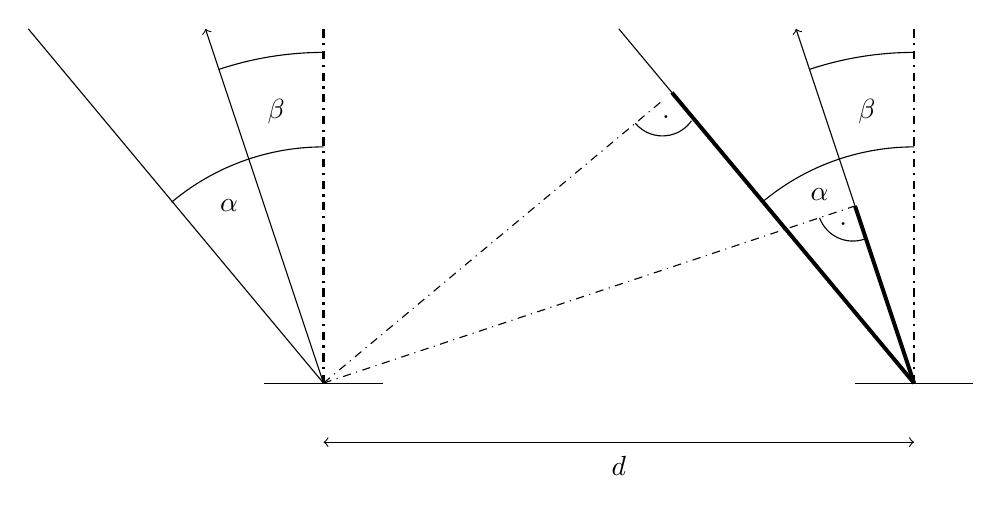
\begin{tikzpicture}[scale=1.5]
    \draw (0,0)--(1,0);
    \draw [thick, dash dot] (0.5,0)--(0.5,3);
    \draw (-2,3)--(0.5,0);
    \draw [->] (0.5,0)--(-0.5,3);
    \draw (0.5,2.8) arc (90:108.5:2.8);
    \draw (0.5,2) arc (90:130:2);
    \draw (0.1,2.3) node {$\beta$};
    \draw (-0.3,1.5) node {$\alpha$};
    \draw (5,0)--(6,0);
    \draw [thick, dash dot] (5.5,0)--(5.5,3);
    \draw (5.5-2.5,3)--(5.5-2.5*0.82,3*0.82);
    \draw [line width=0.5mm] (5.5-2.5*0.82,3*0.82)--(5.5,0);
    \draw [line width=0.5mm] (5.5,0)--(5.5-0.5,0.5*3);
    \draw [->] (5.5-0.5,0.5*3)--(4.5,3);
    \draw (5.5,2.8) arc (90:108.5:2.8);
    \draw (5.5,2) arc (90:130:2);
    \draw (5.1,2.3) node {$\beta$};
    \draw (4.7,1.6) node {$\alpha$};
    \draw [dash dot](0.5,0)--(0.5+2.4*6/5,2.4);
    \draw [dash dot](0.5,0)--(0.5+1.5*3,1.5);
    \draw [<->] (0.5,-0.5)--(5.5,-0.5);
    \draw (3,-0.7) node {$d$};
    \draw (0.5+2.2*6/5,2.2) arc (220:325:0.3);
    \draw (3.4,2.25) node {$.$};
    \draw (0.5+1.4*3,1.4) arc (200:290:0.3);
    \draw (4.9,1.35) node {$.$};
  \end{tikzpicture}
  \caption{Gangunterschied (fett eingezeichnet) für benachbarte Strahlen}
  \label{Gangunterschied}
\end{figure}

\subsection{Balmer-Serie}
Die Energie-Eigenzustände des Wasserstoffatoms werden durch die Quantenzahlen $n,l$ und $m$ beschrieben. Ein Zustand mit der Hauptquantenzahl $n$ hat dabei den Energie-Eigenwert $E_n=-Ry/n^2$, wobei $Ry$ die Rydberg-Energie ist. Wechselt das Wasserstoffatom von einem Zustand mit Hauptquantenzahl $n$ zu einem energetisch niedrigeren Zustand mit Hauptquantenzahl $n'$ wird ein Photon der Energie 
\begin{align}
  E_{n \rightarrow n'}=Ry \left( \frac{1}{n'^2} - \frac{1}{n^2}\right)
\end{align}
emittiert. Die Balmer-Serie enthält alle Frequenzen des Emissionsspektrums, die aus dem Übergang von einem Niveau $n>2$ auf das Niveau $n'=2$ entstehen.

\subsection{Linienbreite}
In der Praxis werden die mit dem Reflexionsgitter beobachtbaren Balmer-Linien eine gewisse Ausdehnung haben, mögliche Ursachen dafür sind:
\begin{itemize}
\item
Im Versuch wird das Spektrum von einem Gemisch aus Deuterium und normalem Wasser in einer Gasentladungsröhre untersucht. Durch die abweichende reduzierte Masse von Deuterium und Wasserstoff ändert sich auch das Emissionsspektrum leicht, so, dass es zu einer Aufspaltung der Linien kommt, der Isotopieaufspaltung.
\item    
Durch die thermische Bewegung der Atome kommt es zur Dopplerverschiebung der Wellenlänge des emittierten Lichtes. Bewegt sich das Atom mit der Geschwindigkeit $v$ auf den Empfänger zu und emittiert ein Photon der Wellenlänge $\lambda$, so misst dieser die Wellenlänge 
\begin{align*}
  \lambda'=\lambda \cdot \left(  1+ \frac{v}{c} \right),
\end{align*} 
wobei $c$ die Lichtgeschwindigkeit ist. Nimmt man an, dass es sich bei dem Gas der Gasentladungsröhre um ein ideales Gas handelt gilt für die Geschwindigkeit $v$ jedes Atoms (mit Masse $m$ und Boltzmann-Konstante $k_\mathrm{B}$)
\begin{align*}
  \frac{1}{2} m v^2=\frac{3}{2} k_\mathrm{B} T.
\end{align*}
Durch die Dopplerverschiebung schwankt die Wellenlänge also im Bereich
\begin{align}
  \lambda'=\lambda\left(1 \pm \frac{1}{c}\sqrt{\frac{3k_\mathrm{B}T}{m}} \right).
\end{align}
\item
Nach \cite{unschaerfe} gilt, dass wenn ein angeregter Zustand des Atoms die mittlere Lebensdauer $\tau$ hat, die Spektrallinie dieses Zustandes die Form einer Lorentz-Kurve mit Breite 
\begin{align}
  \Delta E=\frac{\hbar}{\tau}
\end{align}
hat.
\end{itemize}